\documentclass[11pt]{beamer}
\usepackage{amsmath}
\usepackage{graphicx}
\usepackage{tikz}
\usepackage{array}
\usepackage{pgflibraryshapes}
\usepackage[utf8]{inputenc} 
\usepackage[francais]{babel} 

\makeatletter
\begin{document}

\title[Attaques timings contre les caches des CPU]{\textit{Attaques timings contre les caches des CPU} }

\author[Jean BAUDINAT, Chloé MACUR]{Jean BAUDINAT, Chloé MACUR}

\institute[Télécom ParisTech]
{\scriptsize{Télécom ParisTech\\ \vspace{0.2cm} 
  }
}
\date[\thedate]{\footnotesize{\textsl{SSE} - 22 Juin 2015}}

\begin{frame}
  \titlepage
\end{frame}

\section*{Plan}
\addtocounter{section}{-1}
\begin{frame}{Plan} 
  \tableofcontents%[hideallsubsections]
\end{frame}

%\AtBeginSection[]
%{
%  \begin{frame}<beamer>
%    \frametitle{Plan}
%    \tableofcontents[currentsection,subsection]
%  \end{frame}
%}



\section[Fonctionnement du cache]{Fonctionnement du cache}

\begin{frame}{Fonctionnement du cache}
But: accélérer les calculs (\emph{cache hit}/\emph{cache miss})

\begin{figure}[h]
  \centering
  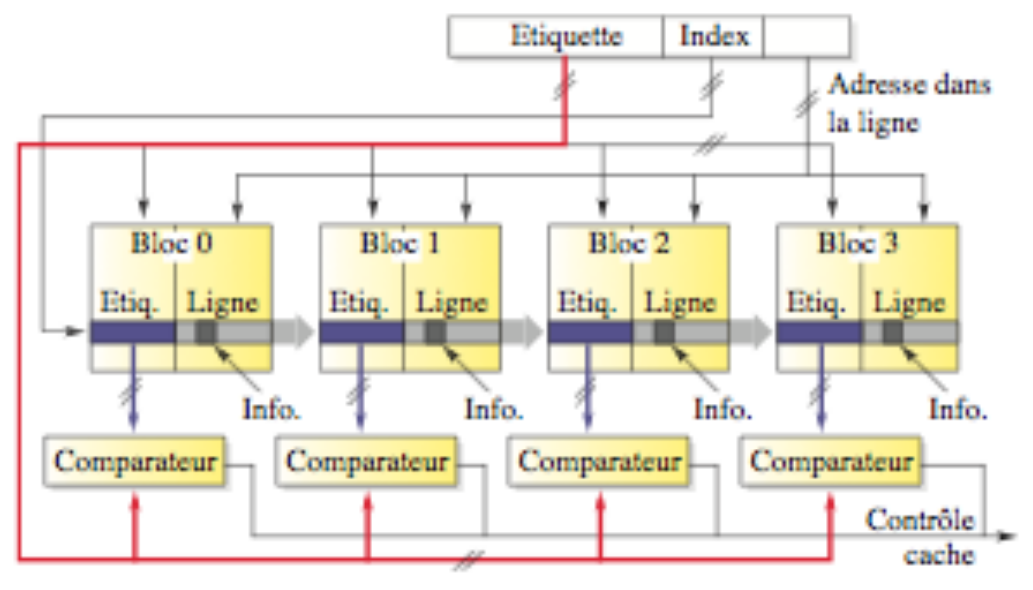
\includegraphics[width=7.5cm]{figures/cache_associative.png}
  \caption{Caches associatifs par blocs (\emph{4-way set associative})}
  \label{cache} 
\end{figure}
\end{frame}

\section{Fonctionnement de l'attaque : l'exemple d'AES}

\subsection{Vulnérabilité d'AES}
\begin{frame}{Vulnérabilité d'AES}
\begin{figure}[h]
  		\centering
  		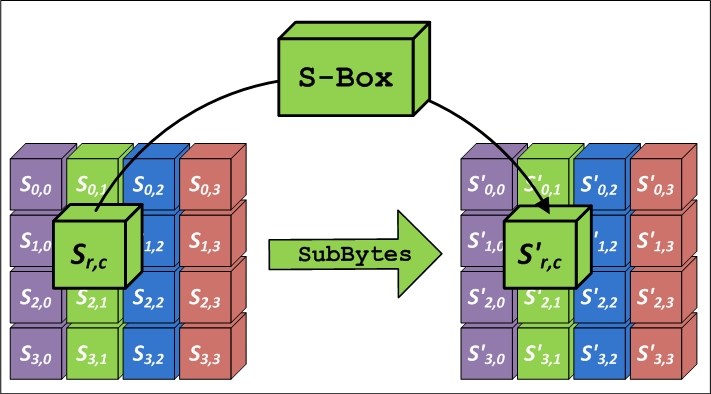
\includegraphics[width=5cm]{figures/s_box.jpg}
  		\caption{S-Box utilisée lors de l'opération SubByte}
  		\label{sbox} 
	\end{figure}
	\begin{itemize}
		\item Boîtes S implémentées sous forme de \emph{Lookup Tables}
		\item Implique différence de temps d'accès selon \emph{Lookup Table} en cache ou non
		\item Différences mesurables
	\end{itemize}
\end{frame}

\subsection{Modèle d'attaquant}
\begin{frame}{Modèle d'attaquant}
	\begin{itemize}
		\item \emph{Time Driven Attack}
			\begin{itemize}
				\item Mesure du temps total d'accès au cache
			\end{itemize}
		\item \emph{Trace Driven Attack}
			\begin{itemize}
				\item Connaissance de l'ensemble de la séquence \emph{hit/miss}
			\end{itemize}
		\item \emph{Access Driven Attack}
			\begin{itemize}
				\item Connaissance des lignes de caches accédées
			\end{itemize}
	\end{itemize}
	
	
\end{frame}

\section{Mise en place concrète de l'attaque}

\subsection{État initial du cache}
\begin{frame}{État initial du cache}
Le cache~\cite{canteaut2006understanding}:
\begin{itemize}
\item Ne contient pas de tables utiles pour le chiffrement (cache flush, par exemple en coupant l'alimentation)
\item Est rempli par l'attaquant (nécessite un accès au cache et donc un système multi-utilisateurs) 
\item Contient déjà toutes les tables nécessaires au chiffrement (temps constant)
\end{itemize}
\end{frame}

\subsection{Attaques synchrones et asynchrones}
\begin{frame}{Attaques synchrones et asynchrones~\cite{osvik2006cache}}


\begin{description}
\item [attaques synchrones]~\\ 
\begin{itemize}
\item attaque en même temps que le chiffrement
\item forge des requêtes de chiffrement (ex: VPN)
\end{itemize}
\item [attaques asynchrones] ~\\
\begin{itemize}
\item bonne connaissance de l'architecture considérée
\item très bons résultats
\item identifier des patterns d'accès à la mémoire réalisés par les autres processus
\item comparaison des statistiques d'utilisation
\end{itemize}
\end{description}

\end{frame}

\subsection{Mesure du temps}
\begin{frame}{Mesure du temps~\cite{osvik2006cache}}

\begin{description}
\item [Evict + Time]  ~\\
\begin{itemize}
\item Chiffrement d'un texte clair
\item Eviction du cache en accédant à d'autres données en mémoire
\item Ssecond chiffrement du même texte clair et mesure du temps
\end{itemize}
\item [Prime + Probe]  ~\\
\begin{itemize}
\item remplissage cache avec données connues
\item chiffrement d'un texte clair
\item lecture des adresses mémoires et mesure du temps
\end{itemize}
\end{description}
\end{frame}

\section{Contre-mesures}

\subsection{Une attaque sur x86 plus difficile}
\begin{frame}{Une attaque sur x86 plus difficile}
	\begin{itemize}
		\item x86 : Architecture parmi les plus répandues
		\item 2010 : Intel crée nouveau jeu d'instruction : AES-NI
		\item Rend totalement impossible attaque
		\item Encore faut-il utiliser ces nouvelles instructions
	\end{itemize}
\end{frame}

\subsection{Une évolution des technologies créatrice de difficultés supplémentaires}
\begin{frame}{Une évolution des technologies créatrice de difficultés supplémentaires}
\begin{figure}[h]
  \centering
  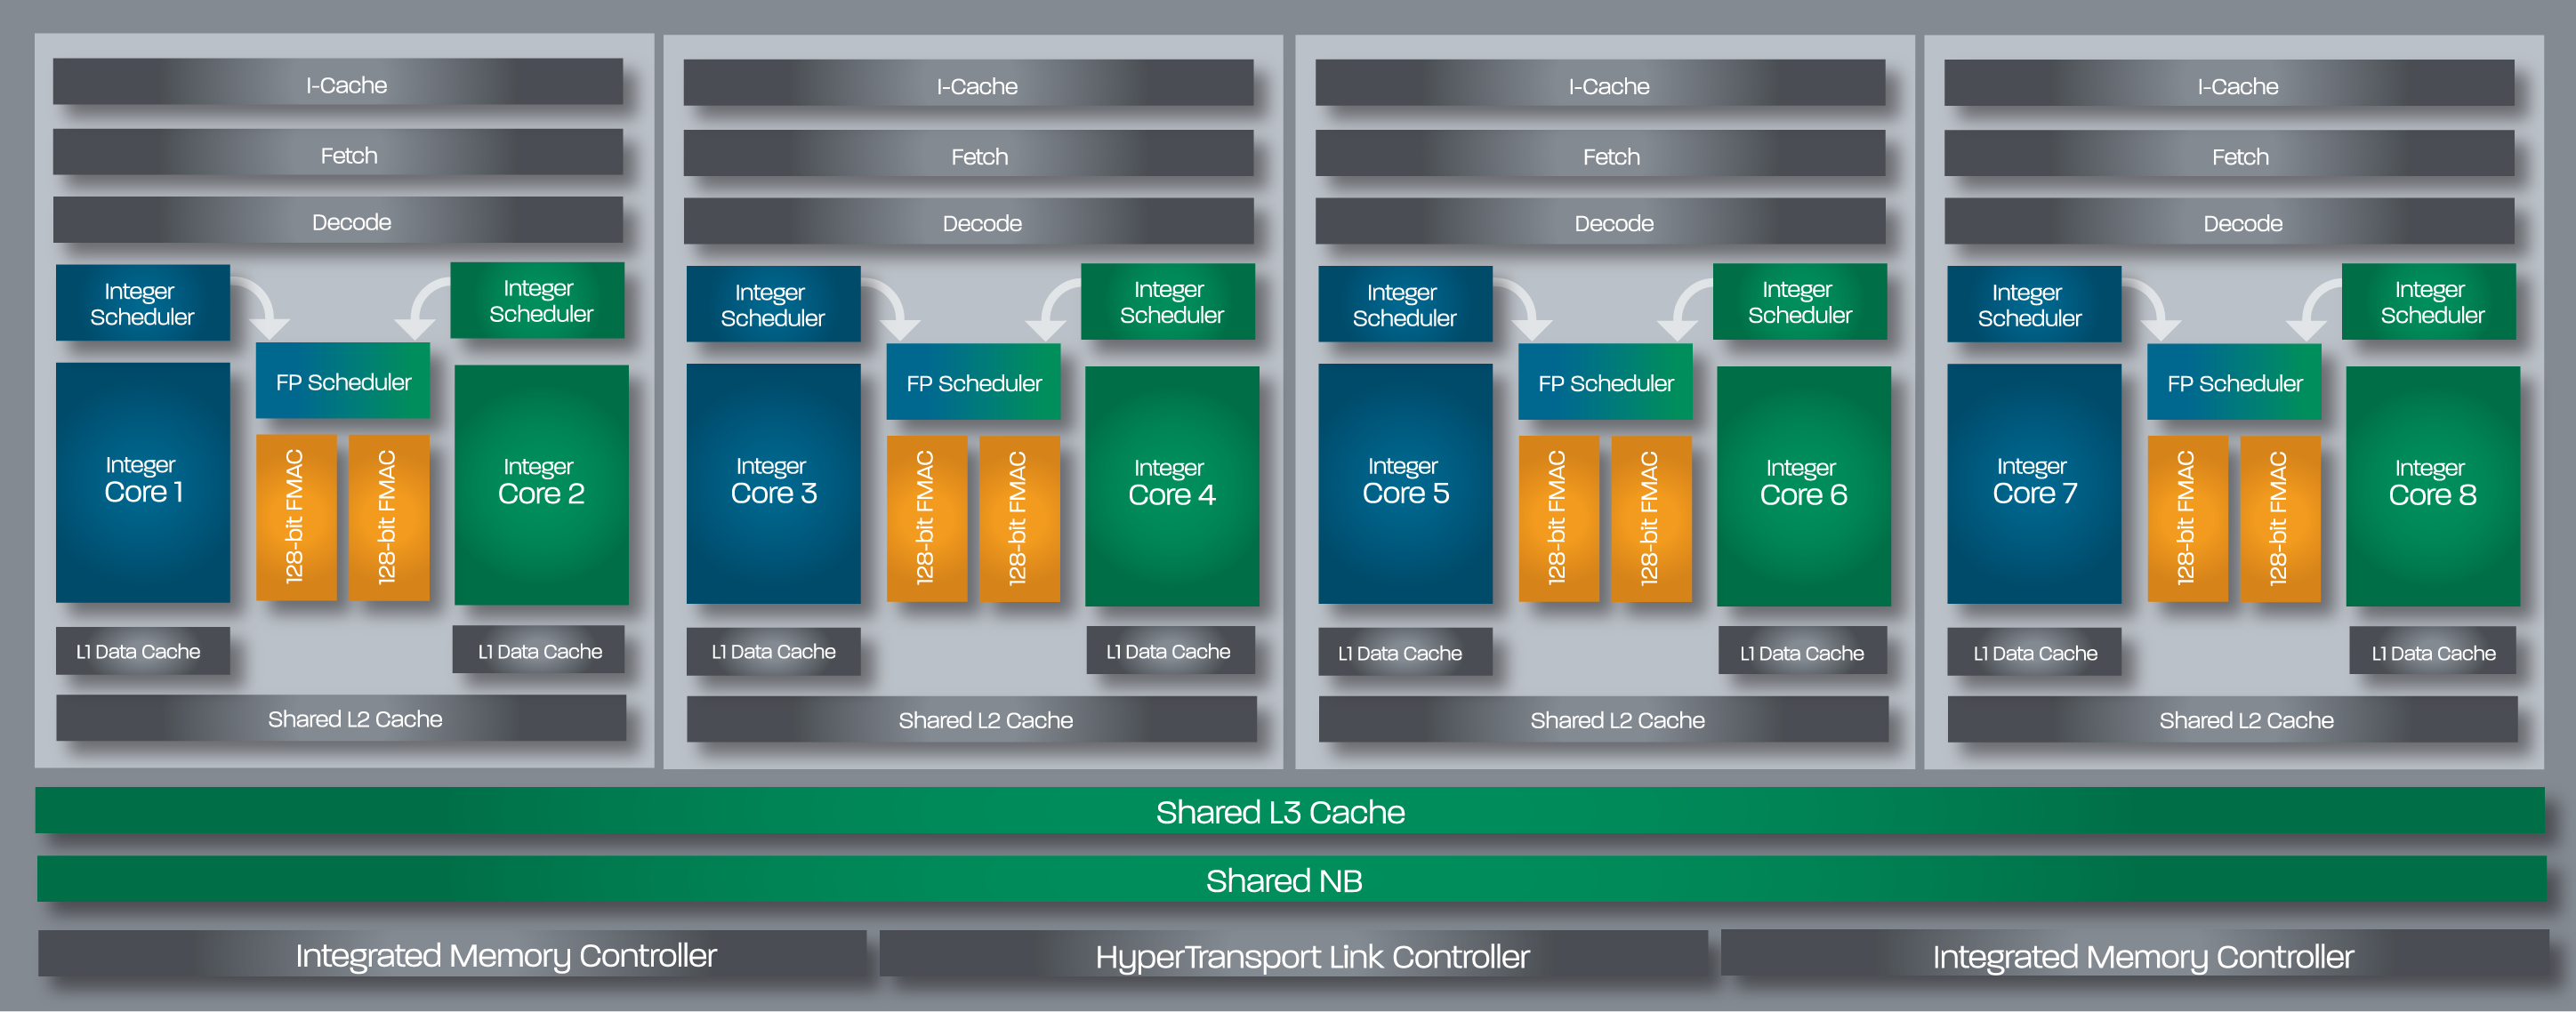
\includegraphics[width=11cm]{figures/BDArch.png}
  \caption{Étagement des caches dans un processeur quadricoeur}
  \label{etagement} 
\end{figure}
\end{frame}

\subsection{Implémentation d'un algorithme en temps constant: le cas d'AES}
\begin{frame}{Implémentation d'un algorithme en temps constant: le cas d'AES}
\begin{itemize}
\item Remplacer les instructions conditionnelles par des séquences d'instruction déterministes~\cite{kasper2009faster}
\item Désactiver le multithreading pour empêcher mesures logicielles
\item Désactiver le cache (ou \emph{no-fill})
\end{itemize}

\begin{description}
\item [Problème:] si on n'utilise pas les boîtes~S ou le cache, mauvaises performances
\item [Solution:] conserver les boîtes~S dans le cache à tout moment
\end{description}
\end{frame}

\begin{frame}{Implémentation d'un algorithme en temps constant: le cas d'AES}
\begin{description}
\item [Méthodes:]~\\
\begin{itemize}
\item Ajout d'une instruction qui charge une table en un nombre constant de cycles~\cite{bernstein2005cache}
\item Matériel cryptographique adjacent en mémoire
\item Éviter interruptions au niveau noyau
\end{itemize}
\item[Autres solutions:] ajout de bruit (chiffrement inutile en parallèle)
\end{description}
\end{frame}


\section*{Conclusion et  références}
\frame[allowframebreaks]{

\begin{block}<+->{Conclusion}
\begin{itemize}
\item Contre-mesures difficiles à réaliser sans \alert{baisse de performance}
\item Utilisation d'une puce cryptographique
\end{itemize}
\end{block}
\vspace{1cm}
\bibliographystyle{plain}
{\tiny \bibliography{ref}}
}

\end{document}
